\chapter{Client}
\label{Client}


\section{Aufbau des Clients}

Der Client wird verwendet, um mit der Datenbankanwendung per REST-API kommunizieren zu können. Er basiert auf einer Shell-Anwendung. Somit kann gezielt und schnell eine Datenanfrage über die Kommandozeile losgelöst werden.
Im folgenden wird auf die Architektur des Clients eingegangen und anschließend ein Anwendungsfall als Beispiel erklärt.

\subsection{Architektur}

Der Client basiert auf dem Spring Shell Framework, das als Grundlage für eine interaktive Kommandozeilen-Anwendung dient. \cite{Spring:SpringShell}
Hier können verschiedene Kommandozeilen-Befehle auf interne Methoden in der Anwendung gemapped werden.\\

Da die verschiedene Methoden auf die REST-API zugreifen müssen, wird hier mithilfe einer \texttt{HTTPClient}-Klasse verschiedene GET- und POST-Requests ausgelöst, die die Datenbankanwendung entgegen nimmt.


\subsection{Anwendungsfall}

Vorerst muss auf Seiten des Servers die Datenbankanwendung eingerichtet werden. Dazu liegt eine bootable Jar-Datei im Gitlab-Repository. \cite{Gitlab:hhu}\\
Um die Jar-Datei auszuführen reicht folgender Befehl:

\begin{center}
\code{sudo java -jar datenbankanwendung.jar -{}-db.root=/tmp}
\end{center}

Der Parameter \texttt{db.root} beschreibt den Ordner, an dem sich eine oder mehrere Dump-Dateien befinden. Die Datenbankanwendung scannt diesen und ermöglicht es dem Client eine Liste aufzurufen und aus diesen, den zu initialisierenden Dump, auszuwählen. Per Default wird das \texttt{/tmp}-Verzeichnis geprüft.

Im gleichen Ordner, liegt ebenfalls eine \texttt{client.jar}, die als Argumente einen Host, sowie einen Port, der auf die Datenbankanwendung zurückzuführen ist, übergeben bekommt.

\begin{center}
\code{sudo java -jar client.jar -{}-db.port=8080 -{}-db.host=localhost}
\end{center}

Sobald die Datenbankanwendung und der Client ausgeführt wurden, kann im Client der Befehlt \textbf{help} ausgeführt. Unter der Überschrift \texttt{Database Commands} befinden sich alle nötigen Befehle, die für die Initialisierung und das Absenden von Anfragen benötigt werden.

\begin{figure}[h]
  \centering
  \begin{subfigure}[b]{1.0\textwidth}
    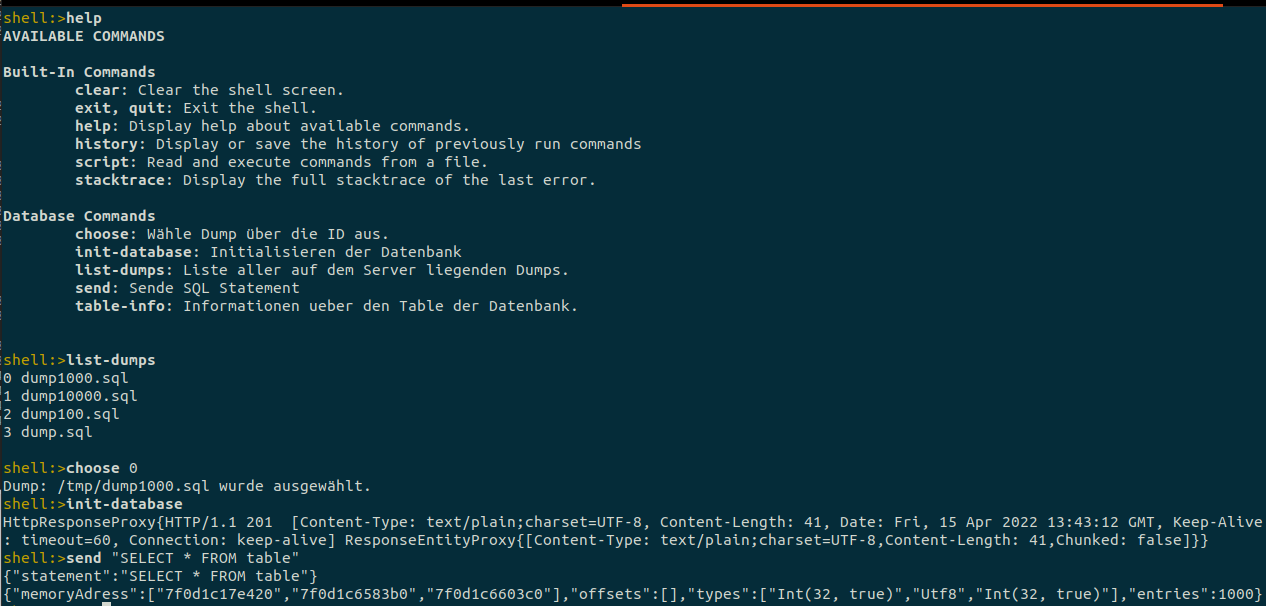
\includegraphics[width=1.0\linewidth]{img/client}
  \end{subfigure}
  \caption{Clientanwendung Beispiel}
  \label{graf_9}
\end{figure}


Um beispielsweise ein Statement abzusenden, kann folgender Befehl verwendet werden:

\begin{center}
\code{send \grqq{}SELECT * FROM table\grqq{}}
\end{center}

Es muss jedoch darauf geachtet werden, dass die Datenbankanwendung erstmalig mit einem richtigen SQL-Dump initialisiert wurde. Als Antwort auf eine abgeschicktes Statement, wird hier die \texttt{IndexResponse} in Form eines JSON-Strings zurückgeliefert. Dies Dient zur Demonstration für den späteren Gebrauch von RDMA.



